% 2024年北京高考数学第10题解析图1：曲线与直线围成区域
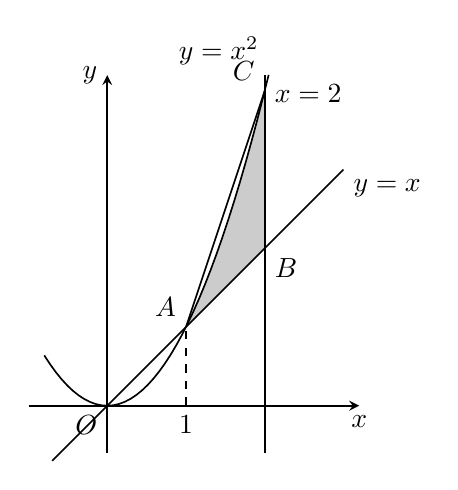
\begin{tikzpicture}[>=stealth,line width=0.6pt,font=\normalsize]
  \draw[->] (-1.0,0) -- (3.2,0) node[below] {$x$};
  \draw[->] (0,-0.6) -- (0,4.2) node[left] {$y$};
  \node[below left] at (0,0) {$O$};

  % 阴影区域: 1 <= x <= 2, x <= y <= x^2
  \fill[gray!40] (1,1) -- plot[domain=1:2,samples=30] (\x, {\x*\x}) -- (2,2) -- cycle;

  % 抛物线 y = x^2
  \draw[domain=-0.8:2.05,samples=40] plot (\x, {\x*\x}) node[above left] {$y=x^2$};

  % 直线 y = x
  \draw (-0.7,-0.7) -- (3.0,3.0) node[below right] {$y=x$};

  % 垂线 x = 2 与 虚线 x = 1
  \draw (2,-0.6) -- (2,4.2) node[below right] {$x=2$};
  \draw[dashed] (1,0) node[below] {$1$} -- (1,1);

  % 点标注
  \coordinate (A) at (1,1);
  \coordinate (B) at (2,2);
  \coordinate (C) at (2,4);

  \draw (A) -- (C);

  \node[above left] at (A) {$A$};
  \node[below right] at (B) {$B$};
  \node[above left] at (C) {$C$};
\end{tikzpicture}
